% !TEX root = ../../book.tex
\chapter{Market Impact Models\label{chap:ch_mi_models}}
\section{Introduction}

Market Impact (MI in short) is the single most important concern in trading. It is also the least understood. It is something every trader experiences but it cannot be easily measured a priori (only the execution costs are directly observed) but can be only estimated ex-post and even then far from any accuracy. We can broadly identify  where it comes from  and we intuitively sense that we can, at least partially, control it through our trading approach but we really don't fully understand its dynamics and how to alter it.


To complicate matters further, large scale trading decisions most often arise from an expectation of price momentum. This means that trading will often occur in the presence of market drift (alpha) and the realized execution cost will be a combination of alpha and the price impact. In ex-post analysis how to decompose  the alpha from the expected impact is extremely arduous, if at all possible, and it is a particularly a constant concern of any quantitatively driven trading (and not) investment as it is critically important to achieve optimal execution. For instance, if we find that most of the cost is due to price drift, the best option would be to accelerate the trading and paying more in impact to capture the more attractive prices. Conversely, if the cost is mostly driven by impact then it would behoove us to slow down our trading to minimize the impact.


Additional complications are due to the complexity of the market structure with its different trading modes (continuous trading, auctions, etc) and types of venues (lit venues, gray pools, dark pools). This requires an ability to measure the differential impact of trading in a particular way in a particular avenue if one hopes to optimally access that liquidity.


Unlike many other practical topics outlined in this book, MI or price impact (PI) has been extensively studied by academics for decades on its own or as part of the more general problem of Optimal Execution which is covered in the next chapter. Unfortunately, the research is somewhat abstract, stylized and is mathematically cumbersome that it has only marginally (and very slowly at that) impacted (pun intended) the consideration by traders and portfolio managers. More than thirty years since the seminal work by Kyle (1985)~\cite{kyle1985} that launched the large body of work on market impact in the industry, the most often used transaction cost model (model estimating the expected cost of an order implicitly incorporating market impact) is the Bloomberg TCA, a simple heuristic and (as far as anybody can tell) un-calibrated model of the form
        \begin{equation} \label{eq:bb_tca}
        \text{TC} = 0.33\, \sigma \sqrt{\frac{Q}{ADV}} + 0.5 \,\text{ba}_{\text{sp}},
        \end{equation}
where $Q$ is the order size, $ADV$ is the average daily volume, $\sigma$ is the stock volatility and $\text{ba}_{\text{sp}}$ is the average bid-ask spread. 


This chapter cannot hope to cover this important topic in any great detail, but it will strive to build an intuition of the drivers of MI that the reader can expand upon. It will then introduce the reader to the most common approaches to market impact modeling used in practice with some insight on how to calibrate them. The chapter will end with a historical review of the most relevant theoretical and empirical research in the area of market impact to benefit the readers. 



% What is Market Impact
\section{What is Market Impact}


There are several definitions of market impact, some are more insightful than others. One that is general and more intuitive is:
        \begin{displayquote}
        \textbf{Market Impact is the cumulative market-wide response of the arrival  of new order flow.}
        \end{displayquote}


This definition incorporates the effect of both trades and order submission (or cancellation). It also includes the effects that, while changing the overall system, ``hidden state'' does not immediately lead to a price change. There are several likely components to this response:
        \begin{itemize}
        \item The first is a purely ``mechanical'' one. The removal of liquidity, either via a trade or via a cancellation, can lead to change in the prevailing mid-price.
        \item The next one is ``economic related.'' Any change in the shape of the order book alters the supply/demand sides leading to a re-establishment of local equilibrium price. 
        \item Another component can be called ``speculative.'' A price move may lead participants to expect the initiation (or continuation) of a momentum trend triggering some ``me-too'' trading in the same direction.
        \item Then there is an ``arbitrage'' component where participants try to step in to provide liquidity in prevision of the price move and immediately get out of it at a better price.
        \end{itemize} 


These effects (and others) are then propagated through the system with various levels of feedback loops leading to very complicated ``chaos-like'' macro dynamics. There is also evidence that these effects are amplified by the ``novelty'' of the price move meaning that the behavior can be highly path dependent. 



% Transaction Costs
\section{Transaction Costs}

As discussed, MI is quantity that cannot be directly observed. What is observed are the prices that one pays to execute an order of a certain size, for a particular instrument, over a specified time period. These prices incorporate several different components that can be broadly grouped into several specific categories:

\begin{enumerate}
\item Explicit Costs: These are costs, in theory at least are known in advance. These include exchange fees, clearing cost, taxes, etc.. They also include all the fixed costs for connectivity, for accessing market data, etc.. Part of these costs are independent of how the order is traded and depend only on the number of shares traded and total notional value (e.g. clearing fees, taxes). Other costs are implementation dependent since they depend on the choice of venue (different venues have different fee schedules) and on the decision of what order aggressiveness (in most venues one is charged to take liquidity while receiving a rebate for providing liquidity).

\item Spread Costs: It is often necessary to cross the spread to take liquidity and the price we achieve is thus higher by the prevailing price (usually defined as the mid-point). If we manage to execute passively the spread cost could be negative.

%\item Opportunity Cost: the loss (or gain) incurred due to the order not completing. For example if on trades with limit orders in a trending market the uncertainty in getting executed could lead to an opportunity loss of taking liquidity immediately at better prices before the price moves. On large order scale opportunity cost comes from trader's decision not to trade the full order in one day or fixing a maximum trading price that leads to the order not completing. Assuming the trader will have to eventually complete the order she might find the market conditions to be much worse.

%\item Delay/Slippage costs. It might take time for the trading decision to hit the exchange and by then the sought after liquidity might already have evaporated.
%\end{itemize}

%We then apply a likely simplification. To make things simpler let's just altogether ignore the explicit costs. We also assume that the order is fully traded so in this initial treatment we can ignore opportunity cost as well. We shall see later that MI and Opportunity Cost, in a broad sense, are at the opposite side of the Optimal Execution 'Tug of War' in the sense that an execution strategy cannot optimize both but will need to balance the two with regards to higher level considerations such as expectation of alpha or trading instructions.

\item Exogenous Price Evolution: At the risk of oversimplifying, this is the theoretical price path that would have happened had we not traded.

\item Market Impact, as defined earlier. 
\end{enumerate}



% A Gentle Introduction to Transaction Cost (TC) Modeling
\subsection{A Gentle Introduction to Transaction Cost (TC) Modeling}


We begin a more in depth treatment of the subject by looking at the most commonly used TC models: Average TC models. These are macro level models that estimate the cost broadly as a function order and execution strategy characteristics. We simplify the picture to focus on the most important aspects: we ignore all the explicit costs and the exogenous price evolution. This last part is an oversimplification but can be rationalized by a few assumptions:
        \begin{itemize}
         \item We are interested in an expected transaction cost thus assuming that we look at average costs over many orders.
         \item Prices behave, to a large extent as random walks.
         \item We assume that the arrival of orders is uncorrelated to the specific price trajectory on the day of trading. 
         \end{itemize} 


Under these assumptions the price evolution accounts only for uncorrelated noise in the cost estimate and can be ignored. Thus in our simplified framework for transaction cost we have two remaining components: market impact and spread costs. 
        \begin{equation} \label{eq:tc_1}
        \text{TC}= f(\text{mi},\text{sc})
        \end{equation}


In most cases, an additional simplification is made in that the two components are additive:

        \begin{equation}\label{eq:tc_2}
        \text{TC}= \text{mi} + \text{sc}
        \end{equation}


Let us start with the simpler component: Spread Costs. As the name implies, this cost is due to crossing the spread on a portion of the order. If we were crossing the spread every time we trade this component could be modeled as half the average bid ask spread $\text{ba}_\text{sp}$. In general, during the execution of an order, we will sometime trade aggressively where we incur the half spread and sometime trade passively where we are paid the half spread. Since execution strategies are by definition liquidity demanding, the ratio will be tilted towards the aggressive trading. Thus, the most basic spread cost can be modeled as a portion $\beta$ of $\text{bs}_\text{sp}$. That is usually where the practitioner stops. If we wanted to look deeper, we could note that the spread cost depends on other features. For example, it seems intuitive that if there is more urgency, the more often the trader will be willing to cross the spread. Thus, the spread cost could also be a function of an urgency parameter, often proxied by the average trading rate. Once we incorporate bid-ask spread and the trading rate, we can, as a first approximation, assume that the spread cost is not dependent on other stock and order characteristics. Thus,

        \begin{equation}\label{eq:tc_3}
        \text{TC}= \text{mi} + \beta \text{ba}_{\text{sp}}
        \end{equation}


We turn our attention to the average market impact. Clearly, the size of the order $Q$ is the primary driver of market impact. As we discussed in Chapter~\ref{chap:ch_news_an} size alone it is less explanatory as 100,000 shares of a ultra liquid stock will certainly have less impact than an illiquid stock that trades only 200,000 shares per day. So a normalized order size $\frac{Q}{\text{ADV}}$ is usually used. Additionally it is well known that, all else being equal, the more volatile the stock is the more the expected cost. What is the intuition here? One way to think about it is that volatility (and spread to some extent) is a measure of  uncertainty around the ``true'' value of the stock. One would then expect that the effects of ``sensing'' a large order in the market would be magnified. Note that volatility is correlated to spread, and so higher volatility stocks will have a higher spread cost.


A more general average TC model is
        \begin{equation}\label{eq:tc_3}
        	\text{TC}= f \big(\frac{Q}{\text{ADV}}\,,\, \sigma \big) + \beta \,\text{ba}_{\text{sp}}.
        \end{equation}
What does the function $f$ look like? Most models assume a multiplicative relationship with power law relationship for both relative size and volatility:
        \begin{equation}\label{eq:tc_3}
	\text{TC}=\alpha  \sigma^{\delta} \left( \frac{Q}{\text{ADV}} \right)^{\gamma}.
        \end{equation}
It is a well studied fact in MI research that the exponent $\gamma$ for relative size is less than one (relatively) well approximated by $0.5$ and thus `$f$' is a square root law. This is an empirical fact and there are several theories for why this is the case. See Gatheral (2010)~\cite{gatheral} for a discussion about this. The square root formula implies that the cost of trading is independent of time taken to liquidate. If ADV and $\sigma$ are fixed, the price impact depends only on the trade size. For the exponent $\delta$ of volatility there is some debate and the data seem to point that the model is somewhat mis-specified. On one hand, there is some evidence that a stock twice as volatile is twice as expensive to trade, so many models have $\delta = 1$. On the other hand when one looks at it over time, and compare average costs in different volatility regimes it has been shown that if the whole market where to dramatically increase in volatility, like at the height of the 2008 financial crisis, the average cost did not increase by the same amount. They jumped by about \todo{(NEED NUMBER)} indicating that $\delta < 1$. Although it is not noted elsewhere, one way to account for that would be to use two measures of volatility: overall market  $\sigma_M$ with an exponent less than 1 and relative volatility $\frac{\sigma}{\sigma_M}$ that has exponent of 1. The most common approach is to re-calibrate the model over time fixing $\delta=1$ and allowing varying $\alpha_t$ to absorb the effect of any regime change. We thus come to the ``standard'' functional form for a TC model:

        \begin{equation}\label{eq:tc_3}
	\text{TC}= \alpha  \sigma \sqrt{\frac{Q}{\text{ADV}}} +  \beta\, \text{ba}_{\text{sp}}.
        \end{equation}


For many years, traders have used this simple sigma-root-liquidity model described for example by Grinold and Kahn (1994)~\cite{grin2000}. The model \eqref{eq:tc_3} stated in another form:
	\begin{equation} \label{eqn:spreadcost}
	\text{TC} - \text{Spread Cost} = \alpha \cdot \sigma \sqrt{\dfrac{Q}{\text{ADV}}},
	\end{equation}
Thus the relative size (RS), $\frac{Q}{\text{ADV}}$ is the key factor in the pre-trade cost estimation and the impact is proportional to volatility. The square root of relative size is expected because risk capital should be proportional to the square-root of the holding period. In Toth, Lemperiere, Deremble, Lataillade, Kockelkoren and Bouchaud (2011)~\cite{toth2011anomalous}, the authors present an argument that if latent supply and demand are linear in price over some plausible range of prices, which is a reasonable assumption, market impact should be square-root.


The square-root formula as stated in \eqref{eqn:spreadcost} refers only to the size of the trade relative to daily volume. It does not refer to for example, the rate if trading, how the trade is executed and the market capitalization of the stock. If the trading is quite aggressive, the square-root formula tends to break down. Moro, Vicente, Moyano, Gerig, Farmer, Vaglica, Lillo and Mantegna (2009)~\cite{moro2009market} observe that the price path during the execution follows a power law:
	\begin{equation} \label{eqn:ptalpha}
	p_t - p_0 = \alpha \cdot \left( {\frac{t}{T}} \right)^{2/3},
	\end{equation}
where $T$ is the duration for the execution of the parent-order. Immediately after completion of a parent-order, the price begins to revert. Models used in industry are mostly functions of the determinants identified above in Equations~\eqref{eqn:spreadcost} and \eqref{eqn:ptalpha}.


The shrewd reader will notice immediately that something is amiss. We have discussed that MI and thus TCs are highly dependent on the approach used for trading but the standard model does not seem to incorporate anything that accounts for the type of trading strategy. One important reason for this has to do with data availability. To calibrate such a model, we need data that will allow us to calibrate the average effect of the use of a different strategy to trade the same amount of stock over the same amount of time. \todo{To Be Discussed}



\subsection{Calibration of a simple TC model}


% Historical Review of Market Impact Research
\section{Historical Review of Market Impact Research}

\todo{TO BE CLEANED UP}


As we had discussed at the beginning of this chapter, one of the main focuses of Algorithmic Trading is to minimize costs of execution. When a large order is executed in the market, it causes market impact (MI), which is commonly defined as the deviation of the post-trade market price from the market price that could have prevailed had the trade not occurred (Fabozzi, Focardi and Kolm (2006)~\cite{ffk}). To alleviate MI and the implied transaction cost (TC), a trader may use an algorithmic trading system to slice a large ``parent'' order into a sequence of ``child'' orders. While a slicing strategy is typically motivated by the liquidity constraint associated with executing a large order in one print, it is usually balanced against the risk and opportunity costs associated with the execution of a sequence of child orders over a longer duration as discussed earlier.


In asset management, with the competitive focus of the industry on cost management and with the diminishing returns of crowded strategies, understanding and managing MI has become a crucial component of a systematic investment process. For an estimate of its size among the transaction costs that include explicit costs such as brokerage commissions and fees, see Table~\ref{tab:empttrans} from Berkovec and Heidle (2010)~\cite{borkoheidle}. Managing MI has important implications on three aspects of algorithmic trading: pre-trade TC estimation, post-trade TC analysis and the design of optimal trading strategies (Almgren (2008)~\cite{alm2008}). The post-trade analytics provides a necessary diagnostics for a client to reflect on the choice of trading strategies as well. 

	\begin{table}[!ht]
	\caption{Empirical Transaction Cost Estimates$^1$ \label{tab:empttrans}}	
	\begin{tabular}{|c|c|c|}
	Type & Fixed & Variable \\ \hline \hline
	Explicit & Commissions (7.4bp) & Bid-ask spreads (1.9bp) \\ \hline
	& Fees & Taxes \\ \hline \hline
	Implicit & & Delay Cost (9.5bp) \\ \hline
	& & Price Movement Risk \& \\
	& & Market Impact Costs* (35.6bp) \\ \hline
	& & Timing Risk \& Opportunity Costs (11.7bp) \\ \hline 
	\end{tabular}
	{\small *Major Component \\ 1: Readers should note changes in the market that have taken place since these numbers were reported. The commissions are quite expensive for current trading. Most developed markets  have commissions less than 1~bps, while E.M. markets are in the range of 2--5~bps for e-trading. The bid-ask spread makes sense if it is half a spread of liquid U.S. stocks. For other markets, it can be much higher.}
	\end{table}


The study of price impact dates back to Bagehot (1971)~\cite{bagehot} who postulated that the market consists of heterogeneously informed traders. The specialist cannot distinguish between informed and uninformed (liquidity) traders and fixes a spread that can balance the trading cost. The asymmetric information models based on this notion have been extensively studied in finance literature. The traders do convey information and Hasbrouck (1991)~\cite{hasbrouk} provides empirical evidence that the market maker can infer information from the characteristics of the sequence of trades. The seminal work by Kyle (1985)~\cite{kyle1985} and Huberman and Stanzl (2004)~\cite{huberstan} indicate that an order of large size (parent order) must be sliced into a number of small order (child orders) so that the volume per se will not signal informed trading. The hypothesis that time between the trades could convey the information flow (Easley and O'Hara (1992)~\cite{easleyo}) and its impact on price is studied in Dufour and Engle (2000)~\cite{dufour}. Long durations are usually associated with no new news and the variations in trading intensity are taken to be positively correlated with the behavior of the informed traders. \twomedskip


\noindent \textbf{Origins of Market Impact:} Most conventional definitions of the MI of a trade equate it with the deviation of the post-trade market price from the market price that would have prevailed had the trade not occurred. Figure~\ref{fig:marketimpt} shows an idealized MI picture of $n$-share sell order from Fabozzi, Focardi and Kolm (2006)~\cite{ffk} but Figure~\ref{fig:detmarketimpt} is augmented to include other information:
	\begin{enumerate}[(i)]
	\item The state of the order book that establishes a pre-trade equilibrium.
	\item How this equilibrium is disturbed by a market order to sell and shares.
	\item As the sell order depletes the bid order book, it obtains an increasingly lower trade price and results in the trade print, and, 
	\item How over time the price gradually moves up back to recover some of the price drop. 
	\end{enumerate}
Accordingly, the difference between (iv) and (iii) is called temporary impact, whereas the difference between (iv) and (i) is called permanent impact. If we are looking to model the MI effect of sequential trades, as shown in Figure~\ref{fig:marketimpt}, the temporary and permanent impact will be superpositions of those of individual trades. The permanent impact is often assumed to be immediate and linear in the parent trade size, and the post-trade equilibrium to be the same for the order of n shares or a sequence of m orders of n/m shares each (Almgren, Thum, Hauptmann and Li (2005)~\cite{athl}, Fabozzi et al., (2006)~\cite{ffk}). By contrast, the temporary impact is a function of how the ``parent'' trade is split into smaller ``child'' trades.

	\begin{figure}[!ht]
	\centering
	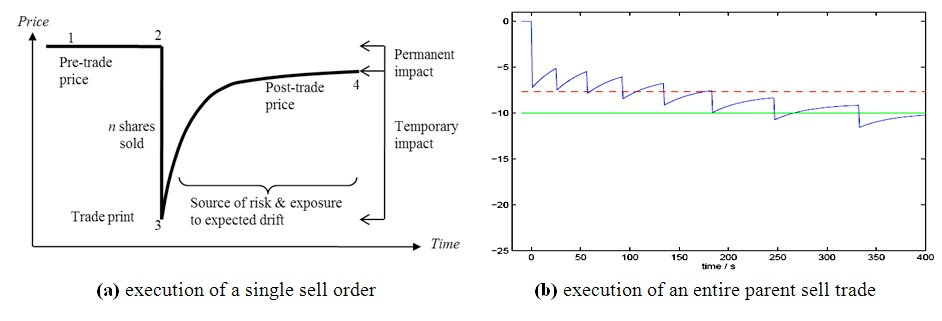
\includegraphics[width=\textwidth]{chapters/chapter_exec_models/figures/fig1ab.jpg}
	\caption{Idealized MI Model: single sell trade (left) and entire parent sell trade (right). \label{fig:marketimpt}}
	\end{figure}


The mechanisms responsible for the permanent and temporary impacts have been a subject of significant interest. One common view links price changes accompanying large trades to the information cost and liquidity cost (Chan and Lakonishok (1995)~\cite{chan1995}; Holthausen, Leftwich and Mayers (1990)~\cite{holthausen1990}) potentially attributed to any transaction. In terms of information cost, the market response to the fact that a market participant has decided to sell (buy) shares of a particular stock could be perceived as conveying new (private) information about the fundamentals of a security, e.g., firm's management, debt conditions, and thus its future prices. Consequently, it results in a permanent price change with no price reversals. In terms of liquidity cost, the market response to the fact that liquidity was removed out of the order book can be perceived as the effect of distorting the liquidity demand/supply equilibrium. The consequence is a temporary price impact that dissipates soon after the trading occurs, at a speed that depends on the market ability to absorb liquidity demand.


Independent of the market microstructure responsible for MI, two central concerns to much theoretical and empirical work are the functional form (shape) of the MI and the key determinants of this form. As seen in Figure~\ref{fig:detmarketimpt}, MI is influenced by trade-related factors (e.g., relative trade size, time and speed of trade), asset-specific factors (e.g., market capitalization, shares outstanding, bid-ask spread) and exchange- and market-related factors (e.g., liquidity, trading volume, institutional features). Models that incorporate these factors tend to be more complex but seem to result in better predictive power.

	\begin{figure}[!ht]
	\centering
	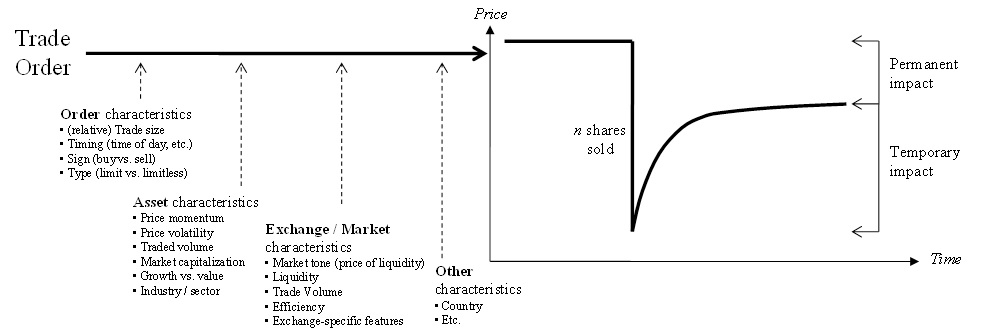
\includegraphics[width=\textwidth]{chapters/chapter_exec_models/figures/fig2.jpg}
	\caption{Determinants of Market Impact. \label{fig:detmarketimpt}}
	\end{figure}



\subsection{Some Stylized Models}	

Numerous stylized MI models offer some insights into possible shapes of the permanent and temporary impact functions. Some of these models focus only on the permanent impact, while some models also attempt to capture the effect of temporary impact. \twomedskip


\noindent \textbf{Equilibrium Permanent Impact Models:} Models of one class, including Kyle's (1985)~\cite{kyle1985} and Hubberman and Stanzl's (2004)~\cite{huberstan}, rest on the efficient market hypothesis positing that all available information gets impounded in prices. These models use a time-independent framework to establish an equilibrium price after a trade is executed. This means that trades are assumed to have only a permanent price impact (Huberman and Stanzl (2004)~\cite[p.1260]{huberstan}).


Under these settings, Huberman and Stanzl (2004)~\cite{huberstan} show that, if no quasi-arbitrage possibilities exist (to ensure viable markets), the permanent impact must be linear in the trade quantity and is symmetric between buys and sells. Linearity in trade size has been established by Kyle (1985)~\cite{kyle1985} as well. In fact, Huberman and Stanzl (2004)~\cite{huberstan} add that ``Nonlinear, time-dependent price-update functions may assume ``chaotic'' shapes without giving rise to price manipulation. Only when additional assumptions are made on the shapes of these functions does the analysis become meaningful.''


Almgren et al. (2005)~\cite{athl} develop a different market impact model, in the context of finding an optimal execution strategy for a large trade [see the discussion of Almgren and Chriss model in Section~\ref{subsec:almchrmodel}] that is sliced into several smaller trades. They describe the random process satisfied by the stock price using an arithmetic Brownian process that depends directly on a permanent impact function that is linear in trade size and therefore has no effect on the optimal execution strategy. However, they recognize that if the total number of units traded is sufficiently large, the execution price may steadily change between trades, in part because the supply of liquidity is exhausted at each successive price level. They assume that this effect is short-lived because liquidity returns after each period and a new equilibrium price is established. They model this effect using a temporary price impact function that is non-linear in trade size. They then postulate that both the permanent and temporary impact functions follow power laws based on the empirical results. (Loeb (1983)~\cite{loeb}; Lillo, Farmer and Mantegna (2003)~\cite{farmermantegna}). \twomedskip


\noindent \textbf{Hybrid Impact and Propagator-Style Models:} Models of another class assume that trading agents have zero intelligence (instead of being fully rational) and take random decisions to buy or to sell, but that their action is interpreted by all the others agents as containing some potential information. The mere fact of buying, or selling typically leads to a change of the ask $a$, or bid $b$, price and hence to a change of the midpoint $p=\frac{a+b}{2}$. The new midprice is also expected to follow a random walk (at least for sufficient large times), if it is immediately adopted by all other market participants as the new reference price around which new orders are launched.


Madhavan et al. (1997)~\cite{madhaven1997} develop a price formation model postulating that the (bid-ask) mid price `$p$' changes because of unpredictable public information shocks (news) and microstructure effects that include statistical effects of order flow fluctuations (e.g., autocorrelation) and trading frictions (e.g., asymmetric information, dealer costs). This postulate automatically removes any predictability in the price returns and ensures market efficiency. If all trades have the same volume and the surprise component of the order flow at the $k$th trade is given by $\epsilon_k - \rho \,\epsilon_{k-1}$, where the signs of trades $\epsilon_n$ are generated by a Markov process with correlation $\rho$,\footnote{This means that the expected value of $\epsilon_k$ conditioned on the past only depends on $\epsilon_{k-1}$, given by: $E(\epsilon_k\,|\,\epsilon_{k-1})=\rho\,\epsilon_{k-1}$.}  one writes the following evolution equation for the midprice as:
	\begin{equation}\label{eqn:midpointdelta}
	\Delta p_{k+1}= p_{k+1} - p_k= \theta[ \epsilon_k - \rho \epsilon_{k-1}] + \eta_k,
	\end{equation}
where $\eta$ is the shock component and the constant $\theta$ measures the size of trade impact. Empirical estimation of their model are not aimed at investigating the shape of impact functions.\footnote{First, both information flows and trading frictions are important factors in explaining intraday price volatility in individual stocks. Second, information asymmetry decreases steadily throughout the day, however, dealer costs increase over the day (possibly reflecting the costs of carrying inventory overnight) so that bid-ask spreads exhibit the U-shaped pattern commonly noted in previous research studies.}


Others extend the model of Madhavan et al. (1997)~\cite{madhaven1997} to gain insight into the shape of impact functions.  Bouchaud et al. (2009)~\cite{bouchaud2009} use \eqref{eqn:midpointdelta} to compute several important quantities. Principally, they write the lagged return impact function (for time points $n$ and $n+l$), denoted $R_l$ as
	\begin{equation} \label{eqn:rlittlel}
	R_l = p_{n+l}-p_n = \theta \sum_{j=n}^{n+l-1}[\epsilon_j - \rho \epsilon_{j-1}]+ \sum_{j=n}^{n+l-1} \eta_j,
	\end{equation}
and then show that the lagged impact function is constant and equal to:
	\begin{equation} \label{eqn:rlittlel2}
	R_l = \theta (1-\rho^2), \quad \forall l.
	\end{equation}
Now define the ``bare'' impact of a single trade taken at time $l$, denoted $G_0(l)$, which measures the influence of a trade at time $n-l$ on the bid-ask midprice at time $n$. Written in terms of $G_0(l)$, the midpoint process is expressed as:
	\begin{equation} \label{eqn:plittlen}
	p_n = \sum_{j=-\infty}^{n-1} G_0 (n - j - 1)\,\epsilon_j + \sum_{j=-\infty}^{n-1} \eta_j.
	\end{equation}
Then it can be shown that $G_0(0) = \theta$ and $G_0(l) = \theta(l-\rho)$ for $l>0$. Bouchaud et al. (2009)~\cite{bouchaud2009} also observe that ``The part $\theta \rho$ of the impact instantaneously decays to zero after the first trade, whereas the rest of the impact is permanent. The instantaneous drop of part of the impact compensates the sign correlation of the trades.''


Bouchaud et al. (2004)~\cite{bouchaud2004} have developed an earlier price evolution model, similar to \eqref{eqn:rlittlel}, where the price at time $n$ is written as a sum over all past trades of the impact of one given trade propagated up to time $n$:
	\begin{equation} \label{eqn:anotherplittlen}
	p_n = \sum_{n'<n} G_0(n - n')\,\epsilon_{n'} \ln{V_{n'}} + \sum_{n'<n} \eta_{n'},
	\end{equation}
where $V_n$ denotes the volume of a trade at time n and $G_0()$ is assumed to be a fixed non-random function that only depends on time differences. The $\eta_n's$ are also random variables, assumed to be independent from $\epsilon_n$, and are used to model all sources of price changes not described by the direct impact of the trades. The authors then consider constraints imposed on the shape of response function, $G_0$, by three empirical results they discuss: (a) the midprice price process is close to being purely diffusive, even at the trade-by-trade level; (b) the temporal structure of the impact function first increases and reaches a maximum after some number (100 to 1000) of trades, before decreasing back with a rather limited overall variation. The sign of the trades shows surprisingly long-range, power-law correlations. These empirical results are reconciled with \eqref{eqn:anotherplittlen} by assuming that the response function $G_0()$ must instead also decay as a power-law in time, with an exponent precisely tuned to ensure simultaneously that prices are nearly diffusive and that the response function is nearly constant. Gatheral (2010)~\cite{gatheral}, assuming that the trading costs should be non-negative, demonstrates that the exponential decay of market impact is compatible only when the market impact is taken to be linear. Thus the debate on the functional form of MI is ongoing. 



\subsection{Models Based on LOB}


It has been noted that the models developed to study market impact generally do not consider situations that may arise from strategies where price impact may depend upon the state of the order book. The second generation models consider the behavior of the limit order book. Hautsch and Huang (2012)~\cite{hauthuang} consider a time-aggregated model. The core activities in the limit order book are captured in Table~\ref{tab:vardef} and the market depth is kept to the three best quotes on both sides of the market.
	\begin{table}[!ht]
	\centering
	\caption{Model \eqref{eqn:7dy} Variable Definitions \label{tab:vardef}}
	\begin{tabular}{ll}
	Variable & Description \\ \hline
	$p_t^a$ & Logarithm of the best ask after the $t$-th event. \\
	$p_t^b$ & Logarithm of the best bid after the $t$-th event. \\
	$v_t^{a,l}$ & Logarithm of the market depth at the $l$-th best ask after the $t$-th event. \\
	$v_t^{b,l}$ & Logarithm of market depth at the $l$-th best bid after the $t$-th event. \\
	$\text{BUY}_t$ & Dummy equal to one if the $t$-th event is a buyer-initiated trade. \\
	$\text{SELL}_t$ & Dummy equal to one if the $t$-th event is a seller-initiated trade. 
	\end{tabular} 
	\end{table}
Let $Y_t$ be a $K$-dimensional listing of the variables in Table~\ref{tab:vardef}; the co-integration model in Chapter~\ref{ch:ch_mvts} is fit for the data:
	\begin{equation} \label{eqn:7dy}
	\Delta Y_t = \mu + \alpha \beta' y_{t-1} + \sum_{t=1}^{p-1} \Gamma_i \Delta Y_{t-i} + u_t.
	\end{equation}
The co-integrating $(K \times r)$ matrix, $\beta$ has first two columns restricted to have entries as zeros except for buy and sell indicators. To study the market impact, the model is written in the reduced-form to capture the impulse-response coefficients as:
	\begin{equation} \label{eqn:7largeyt}
	Y_t = \mu + \sum_{i=1}^p A_i Y_{t-i} + U_t,
	\end{equation}
where $A_1= I_k + \alpha\beta' + \Gamma_1$, $A_i= \Gamma_i - \Gamma_{i-1}$ for $1 < i < p$ and $A_p= -\Gamma_{p-1}$. The $\text{VAR}(p)$ model in \eqref{eqn:7largeyt} can then be written in the form of $\text{VAR}(1)$ as 
	\begin{equation}\label{eqn:starlargeyt}
	Y_t^*= \mu^* + A^* Y_{t-1} + U_t^*,
	\end{equation}
where $\mu^*=(\mu',0',\ldots,0')'$, $Y_t^*=[Y_t',Y_{t-1}',\ldots,Y_{t-p+1}']$, $U_t^*=[U_t',0',\ldots,0']'$ and $A^*=\renewcommand\arraystretch{1.3} \mleft[ \begin{array}{c|c} A_1\cdots A_{p-1} & A_p \\ \hline I_{K(p-1)} & 0 \end{array} \mright]$. It can be shown that 
	\begin{equation}\label{eqn:7anotherlargeyt}
	Y_t= JM_t + \sum_{i=0}^{t-1} JA^i J' U_{t-i},
	\end{equation}
where $J=[I_k,0,\cdots,0]$ is a $k\times kp$ selection matrix and $M_t= A^{*t} Y_0^* + \sum_{i=0}^t A^{*i}U_{t-i}^*$.


Recall that the market impact measures the impact of current trade on the future trades; it is measured by the impulse response function
	\begin{equation} \label{eqn:impulserep}
	f(h,\delta_h) = E[y_{t+h} \,|\, y_t+\delta_y,t_{t-1}, \ldots] - E[y_{t+h} \,|\, y_t,y_{t-i}, \ldots] = JA^{*h} J' \delta_y,
	\end{equation}
where $\delta_y$ is the change to $Y_t$, due to the current trade. The long-run effect, $f(\delta_y)= C \delta_y$, where $C= \beta_\perp(\alpha_\perp' (I_K - \sum_{i=1}^{p-1} \Gamma_i ) \beta_\perp )^{-1} \alpha_\perp'$. Here $\alpha_\perp$ and $\beta_\perp$ are orthogonal to $\alpha$ and $\beta$ in \eqref{eqn:7dy}.


Hautsch and Huang (2012)~\cite{hauthuang} estimate the market impact using the data from Euronext, Amsterdam for heavily traded stocks. The main findings are, besides the existence of co-integrating relationships between quotes and depths, limit orders have long-term effects on quotes, the price movement is influenced by the order size and the decrease of spreads after the arrival of a limit order is reverted back asymmetrically soon after. The between-stock variations in market impact are shown to be related to trading frequency of the stocks. These empirical observations are immensely useful for pre-trade transaction cost estimation.


Cont, Kukanov and Stoikov (2014)~\cite{contkulst} consider the dynamics of market liquidity that is a function of limit orders, market orders and cancellations to model the price impact function. The outstanding limit orders provide a measure of depth in the market on both buy and sell sides and thus also provide a measure of order flow imbalance (OFI). By setting the number of shares (depth) or price levels beyond the best bid and ask is equal to $D$, define the price change in the interval $(t_{k-1},t_k)$ as,
	\begin{equation}\label{eqn:doubleeq}
	\begin{split}
	\Delta P_k^b&= \delta \left[ \dfrac{L_k^b - C_k^b - M_k^s}{D} \right] \\
	\Delta P_k^s&= -\delta \left[\dfrac{L_k^s-C_k^s-M_k^b}{D}\right],
	\end{split}
	\end{equation}
where $L_k^i$, $C_k^i$ and $M_k^i$ for $i=b,s$ denote arrival of the limit orders, cancellations and market orders in the defined interval. Here $\delta$ is the tick size. If $P_k=\dfrac{P_k^b+P_k^s}{2\delta}$, that is mid-price normalized by tick size, for any $s$nd-interval, $(t_{k-1,i},t_{k,i})$, it is postulated that
	\begin{equation}\label{eqn:postulated}
	\Delta P_{k,i} = \beta_i \text{OFI}_{k,i} + \Eulerconst_{k,i},
	\end{equation}
where $\text{OFI}_k=(L_k^b-C_k^b-M_k^s)-(L_k^s-C_k^s-M_k^b)$ and $\Delta P_k=\frac{\text{OFI}_k}{2D}+\epsilon_k$. Here it is important to note that `$\beta_i$' is taken to be price impact coefficient and is taken to be inversely proportional to market depth:
	\begin{equation} \label{eqn:7betai}
	\beta_i=\dfrac{C}{D_i^\lambda} + v_i.
	\end{equation}
The models in \eqref{eqn:postulated} and \eqref{eqn:7betai} can be regarded to represent instantaneous price impact. The model as it can be seen from the set-up assumes that all activities in the limit order book have an average linear impact, $\beta_i$, in the $i$th interval. 


Cont et al. (2014)~\cite{contkulst} using the TAQ data for a month in 2010 for fifty stocks estimate the model in \eqref{eqn:postulated} over ten-second intervals. The model is generally confirmed by the data with $\hat{\beta}_i$ is significant in most of the samples and $\hat{\alpha}_i$ is only significant in less than twenty percent of the samples. It must be noted that there is a significant number of trades posted gets cancelled within a few seconds of submission. Various theories that are postulated (see Hasbrouck and Saar (2009)~\cite{habbrooksaar}) are yet to be fully empirically tested. Hence instead of using OFI, trade imbalance $(\text{TF}_k=M_k^b-M_k^s)$ is used in equation \eqref{eqn:postulated}. Results are still reasonable, but not as strong as using OFI in the model. Finally the relationship between $\hat{\beta}_i$ and $D_i$ (price impact coefficient and depth) is studied; the results indicate for model \eqref{eqn:7betai}, $\hat{C} \sim 0.5$ and $\hat{\lambda} \sim 1$. 


Some interesting conclusions that could be useful for trading are drawn. The impact coefficient varies more with the amount of liquidity provision (OFI) than the trade imbalance (TI). It can be also used to monitor adverse selection. If a limit order is filled after a positive OFI, price is likely to go up and for a limit sell order, a positive change would imply that the order was executed at a loss. These conclusions need to be firmed up with further studies in this area.



% Determinants of Empirical relationship
\section{Determinants of Empirical relationship}


 As noted earlier, key aspect of MI modeling is to provide information about expected pre-trade costs. The studies that have been reviewed on empirical analysis thus far can help us to understand how the price formation and the market impact function evolve during a trading period. But most clients who want to trade large quantities of equities want to know the trading costs a priori. Here we review the relevant studies and augment with our own research in this area. First we review the factors that are found to influence these costs in block trades. Although block trades differ in fundamental ways to algorithmic, they can be treated as all equivalent to a parent trade except that no splitting into child orders occurs.


\begin{itemize}
\item \textbf{Trade Size.} Many studies observe that the (relative) size of trades positively relates to the magnitude of MI (Keim and Madhavan (1996)~\cite{madhavan}), consistent with the prediction of stylized model (Kyle (1985)~\cite{kyle1985}; Huberman and Stanzl (2004)~\cite{huberstan}).

\item \textbf{Market Capitalization.} Keim and Madhavan (1996)~\cite{keim1996}find that the asymmetry of trading costs between buys and sells is more pronounced among smaller stocks. This is consistent with what is broadly known to be the effects of market capitalization on MI (Lillo et al. (2003)~\cite{farmermantegna}; Chan and Lakonishok (1997)~\cite{chan1997}). From a practical point of view, market cap itself may not be a true factor but it can be a proxy for some liquidity characteristics. 

\item \textbf{Price Volatility.} Price volatility has been found to be positively related to MI (Chiyachantana, Jain, Jiang and Wood (2004)~\cite{chiya2004}). One explanation is that elevated volatility is associated with greater dispersion in beliefs, with risk averse traders less inclined to participate in markets, thereby resulting in greater price concessions or MI (Domowitz et al. (2001)~\cite{domo2001})

\item \textbf{Trading Activity.} Dufour and Engle (2000, p. 2467)~\cite{dufour} find that the price impact of trades increases as the time duration between transactions decreases, and more broadly that the price impact is especially large due to increased trading activity, as measured by high trading rates. In their view, ``times when markets are most active are times when there is an increased presence of informed traders; we interpret such markets as having reduced liquidity.'' Likewise, Yang (2011)~\cite[p.91]{yang2011} finds that ``a trade shortly after the previous trade results in higher price impact than one after a long period.'' He also offers ``evidence that increased trading activity (as measured by short durations between trades) is associated with larger price impact, therefore implying a higher degree of information-based trading.''

\item \textbf{Time of Day.} It is reported that the MI for buy trades decreases as time passes during the day, with the highest impact in the first trading hours (Frino, Jarnecic and Leopone (2007)~\cite{frino}).
\end{itemize}


At the higher frequency levels other determinants to consider are:
	\begin{itemize}
	\item Intraday volatility on a 5-min basis
	\item Depth of the order book
	\item Spread
	\item Intraday Price Dynamics
	\item VIX level and return \twomedskip
	\end{itemize}



% Select Empirical Studies
\subsection{Select Empirical Studies}

While there is some discussion about the theoretical models for market impact, published studies based on large scale data are somewhat rare especially when it comes to models useful for pre-trade cost estimation, Almgren et al (2005)~\cite{athl} took US stock trade orders processed by Citigroup for Dec 2001 to June 2003 and estimated a model of the market impact as given in Table~\ref{tab:costimpact}. For two select stocks, IBM and DB, the power law model for market impact are estimated. The temporary impact is defined as $\widetilde{p}_k - p_{k-1}$, for $k$th execution. The model depends on relative size, inverse turnover ratio, which is the number of the shares outstanding to average daily volume and the volatility.


While the square root formula in \eqref{eqn:spreadcost} is quite robust and holds even beyond equity markets, recent empirical studies confirm the need for more general power law functions; the quotient of RS varies depending on other factors that get included in the model (refer to the estimates in Table~\ref{tab:costimpact} for RS). Zarinelli, Treccani, Farmer and Lillo (2015)~\cite{zar} show that logarithmic functional form fits the data better for the large order data that they consider. 


        \begin{table}[!ht]
        \caption{Example of impact costs (Almgren et al. (2005)~\cite{athl} \label{tab:costimpact}}
        \begin{tabular}{lccc}
         & & IBM & DRI \\ \hline
        Average daily volume & ADV & 6.561~m & 1.929m~ \\
        Shares outstanding & $\theta$ & 1728~m & 168~m \\
        Inverse turnover & $\theta/\text{ADV}$ & 263 & 87 \\
        Daily volatility (\%) & $\sigma$ &1.57 & 2.26 \\
        Normalised trade size & $Q/\text{ADV}$ & 0.1 & 0.1 \\ \hline
        Normalised permanent cost & $l/\sigma$ & 0.126 & 0.096 \\
        Perm. price impact (bp) & $l$ & 20 & 22 \\ \hline
        Trade duration (days) & $T$ & 0.1 \hspace{0.2cm} 0.2 \hspace{0.2cm} 0.5 & 0.1 \hspace{0.2cm}0.2 \hspace{0.2cm} 0.5 \\
        Normalised temporary & $K/\sigma$ & 0.142 \hspace{0.2cm} 0.094 \hspace{0.2cm}0.054 & 0.142 \hspace{0.2cm} 0.094 \hspace{0.2cm} 0.054 \\
        Temp. Impact cost (bp) & $K$ & 22 \hspace{0.2cm} 15 \hspace{0.2cm} 8 & 32  \hspace{0.2cm}21\hspace{0.2cm} 12 \\ \hline
        Realized cost (bp) & $J$ & 32 \hspace{0.2cm} 25 \hspace{0.2cm} 18 & 43 \hspace{0.2cm}32 \hspace{0.2cm} 23
        \end{tabular}
        {\small Note: examples of permanent and temporary impact costs are shown, for a purchase of 10\% of the day's average volume, in two different large-cap stocks. The permanent cost is independent of time of execution. The temporary cost depends on the time, but across different assets it is the same fraction of daily volatility (from Almgren et al. (2005)~\cite{athl}); $K= J-I/2$.}
        \end{table}


Limited access to broker-proprietary algorithmic trading data has stifled detailed academic inquiry in this area. While the impact of algorithmic trading is extensively discussed in the finance literature, formal empirical results are rare. The few exceptions we are aware of are: Engle, Ferstenberg and Russell (2012)~\cite{engle2012}, who use proprietary algorithmic trading data from Morgan Stanley to study the risk-return tradeoff associated with increasing the number of child trades and duration of parent trade; Domowitz and Yegerman(2005)~\cite{doye}, who use ITG's Transaction Cost Analysis Peer Group Database to compare execution costs for a set of 40 buy-side clients; and Hendershott and Riordan (2011)~\cite{hernderrio}, who use algorithmic trading data from firms listed on the Deutsche Boerse DAX to measure the contribution of algorithmic trading to price discovery. A few academic studies resort to using proxies based on publicly-available TAQ data. Two examples are: Hendershott et al. (2011)~\cite{hender2011}, who use NYSE electronic message traffic data as a proxy for algorithmic liquidity supply to study how algorithmic trading effects liquidity and bid-ask spreads; and Chaboud et al. (2014)~\cite{chaboud}, who use FX quote data (highest bid and lowest ask) from an electronic limit order book platform called EBS to construct mid-quote series for studying the effect of algorithmic trading on FX rates' volatility. The use of mid-point prices, in the lack of actual arrival price and completion price for a parent trade, has been criticized for failing to capture the possible asymmetry of the bid and ask price impacts of trading, which has been observed to exist for block trades. In any event, none of these studies deals with the estimation of MI models per-se.


Velu, Gretchika, Benaroch, Nehren and Kuber (2015)~\cite{unpub} address these issues using a large algorithmic trading dataset. The data contain ``parent'' algorithmic executions, including the initial arrival price and fill price as well as the child trades' average fill price (computed as the share-weighted average executing price of the child orders). The algorithmic executions are generated using Volume Weighted Average Price (VWAP) and Percent of Volume (POV) strategies.Recall the volume weighted average price (VWAP) strategy schedules to trade some constant percentage of the expected market volume regularly throughout the day, where the proportion traded is adjusted based on historical market volume profiles and the predict volume. Hence, in VWAP, the trading schedule is predetermined based on a prediction of the daily market volume distribution, although the timing of executions may be randomized so as to make the trading pattern less predictable. In any case for efficient execution, it is essential to have good predictive models for volume. 


By contrast, the percent of volume (POV) strategy trades a fixed percentage of the current market volume where the trading schedule is dynamically determined based on a historical analysis of volume profiles used to anticipate trading volumes. Unlike implementation shortfall strategies, VWAP and POV do not explicitly take into account the expected MI in generating their algorithmic executions. Moreover, although firms typically implement proprietary versions of these strategies with parameters reflecting their experience and clients' profiles, VWAP and POV nonetheless generate relatively standardized algorithmic executions. In other words, from the perspective of MI, these two strategies can be safely considered ``plain vanilla'' in the sense that firm-to-firm differences in their behavior and performance are too insignificant. The measures employed, therefore, do not depend on any unique traits of the strategies. The unique aspect of the data is that if the meta order is on the buy side or sell side is explicitly provided. 


The dataset allows us to study the effect of parent characteristics on the market impact and the implied transaction cost (TC). Specifically, we estimate the parameters of a family of power-law models, investigate the explanatory power of different determinants of market impact and TC, and develop insights useable for pre-trade cost estimation. Our model estimation effort is informed by existing stylized market impact models and empirical findings about the market impact of block trades. These stylized models are reviewed earlier in this section. In addition to studying the effects of buy and sell trades, order size, price volatility and market cap, we examine the effect of the number of child trades and duration of the parent trade. Lastly, we also summarize two extensions of our model estimation effort that pertain to the effect of the bid-ask spread on market impact and to the market impact of ETFs traded via algorithmic trading.


This study has some important findings. A central novel insight that emerges from the analysis is that market impact can be substantially decreased by reducing the number of child order trades. There could be several explanations, but a simple plausible one is that reducing the number of child trades reduces the information leakage about trading intentions. This explanation is in line with the main premise of Farmer, Gerig, Lillo, and Waelbroeck (2013)~\cite{farmer2012} that, in an efficient market, market impact is determined by the information that is disseminated through trades. It is also consistent with studies showing that the price impact is larger as the duration between trades decreases and there is increased trading activity (Dufour and Engle 2000~\cite{dufour}; Yang 2011~\cite{yang2011}), and that the number of trades may drive prices more than the actual trade size (Jones, Kaul and Lipson (1994)~\cite{jones1994}).


Another finding is the nuanced difference in market impact and TC that is related to buy and sell trades. On the overall level, this difference is statistically significant, and this presumably contradicts the buy-sell market impact asymmetry commonly reported for block trades. However, a deeper examination reveals a more nuanced difference between buy and sell trades. Visual inspection of the TC vs. trades' relative size and the TC vs stocks market cap shows that in some sub-ranges there is a difference between buys and sells. After dividing trades into 24 bins based on their relative size and testing the TC difference within each bin we observe that the difference is statistically significant in six bins; six out of 24 exceeds the proportion expected when testing multiple hypotheses at a 5\% significance level. Consequently, separate market impact and TC models for buy and the sell trades are estimated, and observed the following about the difference between the coefficients of buys and sells. This difference is significant in models containing a subset of the explanatory factors (e.g., relative size alone, or relative size and volatility), but it is within a two standard errors threshold in models containing all the factors. Our findings notwithstanding, it is necessary to investigate further whether the underlying causes may be linked to the specifics of trade flow, the logic behind many of the trading algorithms.


It is important to mention two caveats . One relates to the role of permanent versus temporary impact in our analysis. The data set does not contain information about the price dynamics after the completion of the parent trades, that is, only completion price for the last child order is available. Therefore, it was not possible to determine what portion of the measured market impact is permanent and what portion of it is temporary. Another caveat relates to the high variability in the data. To obtain a better signal out of the noisy data, the data was smoothed through binning and extraction of key descriptives. The models are based on these descriptives. Nevertheless, for robustness testing all models were estimated using the raw unsmoothed data and the results are qualitatively similar, albeit the $R$-square values are understandably much lower. \twomedskip


\noindent\textbf{Select Empirical Results:} The market impact is modeled as a non-linear function of several stock-related and trade-related factors. The power law form is generally recommended for non-linear shape. The data analyzed in Velu et al. (2015)~\cite{unpub} consists of over 250,000 parent orders fully executed over a one-year period, Oct 1, 2009--Sept 30, 2010. All trades were completed within a single trading day. Each parent order was sliced into multiple child trades; each child trade was executed in one or several partial fills. Only parent trades executed through widely used VWAP (volume-weighted average price) or POV (percent of volume) strategies (Brandes, Domowitz, Jui and Yegerman (2007)~\cite{brandes2007}). This ensures that the participation rate is well-defined and stays roughly constant over the duration of the parent trade. We define 
	\[
	\begin{split}
	\text{Market Impact (MI) in bps }&= \text{side } \cdot \left(\dfrac{\text{\small Completion Price} - \text{\small Arrival Price}}{\text{\small Arrival Price}}\right) \cdot 10000 \\
	\text{Transaction Cost (TC) in bps}&= \text{side } \cdot \left(\dfrac{\text{\small Average filled Price }-\text{ \small Arrival Price}}{\text{\small Arrival Price}} \right) \cdot 10000 \normalsize,
	\end{split}
	\]
where the arrival price is the price when the first child order is executed and completion price is the price when the last child order is executed. Every trade in this data is explicitly identified as buy or sell. This contrasts with studies that use TAQ data that do not have the same explicit identification. Using Lee and Ready (1991)~\cite{leeready} heuristic rule to determine the trade direction can be sometimes inaccurate (Asquith, Oman and Safaya (2011)~\cite{asquith2010} and Chakrabarty, Moulton and Shkilko (2012)~\cite{chakrabarty2012short}). To make the analysis robust, we binned the explanatory variables and obtained smoothed averages; the analysis is based on binned data.


Results start with a visual inspection of the relationships. The graphs clearly indicate that the relationship between MI and RS is non-linear, and it remains non-linear with binning of other factors as well. The relationship between MI and relative size is monotonic till the relative size reaches 20\% or so (Figure~\ref{fig:miandrsplot}).Trades with longer durations clearly have a lower MI (Figure~\ref{fig:mivsrs}). Trades for higher volatility stocks, too, can be read to have a higher MI (Figure~\ref{fig:mivsrs}). Trades on larger market cap stocks have a smaller MI (Figure~\ref{fig:mivsrs}). Lastly, MI becomes higher as the number of child trades increases (Figure~\ref{fig:mivsrs}). This last relationship is important and deserves special attention particularly when designing execution strategies. There is a clear trade-of between low ``immediate'' liquidity impact of small child orders and long term information leverage of the parent order level when hitting the market too frequently. But the power law model is more general and can accommodate interaction effects as well. These graphs for various factors besides RS can be collapsed into a master curve, with appropriate normalization, as given in Lillo et al. (2003)~\cite{farmermantegna}.
	

	\begin{figure}[!ht]
	\centering
	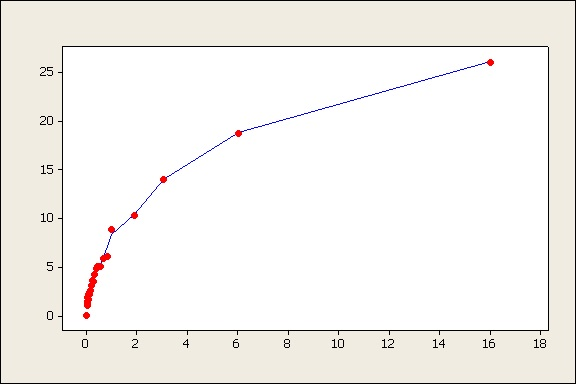
\includegraphics[width=0.9\textwidth]{chapters/chapter_exec_models/figures/fig3.jpg}
	\caption{MI vs. RS. \label{fig:miandrsplot}}
	\end{figure}


    \begin{figure}[!ht]
        \begin{minipage}[b]{0.45\linewidth}
            \centering
            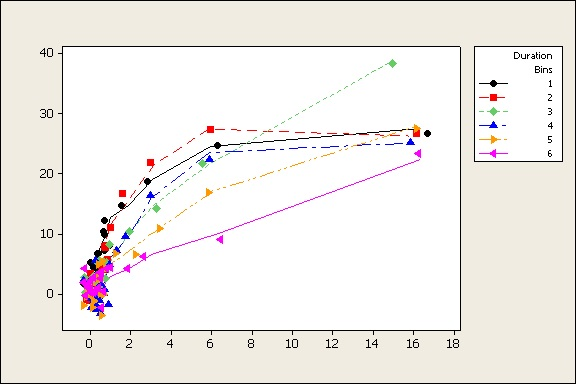
\includegraphics[width=\textwidth]{chapters/chapter_exec_models/figures/fig4.jpg}
            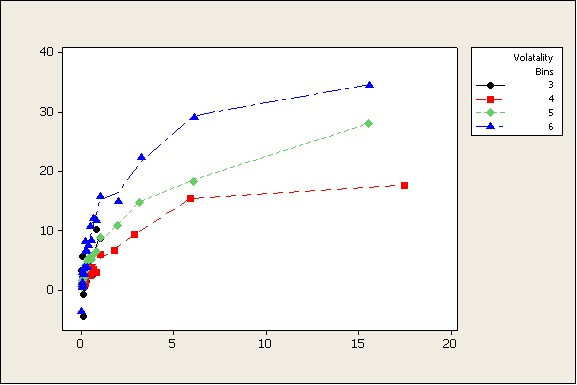
\includegraphics[width=\textwidth]{chapters/chapter_exec_models/figures/fig5.jpg}
        \end{minipage}
        \hspace{0.5cm}
        \begin{minipage}[b]{0.45\linewidth}
            \centering
            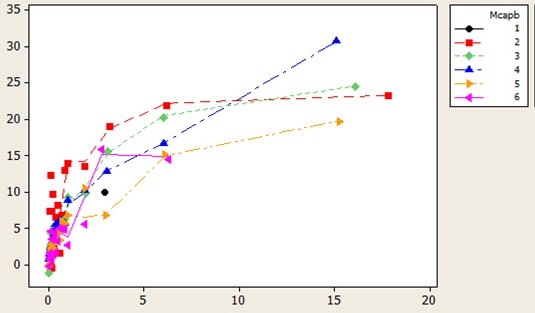
\includegraphics[width=1.05\textwidth]{chapters/chapter_exec_models/figures/fig6.jpg}
            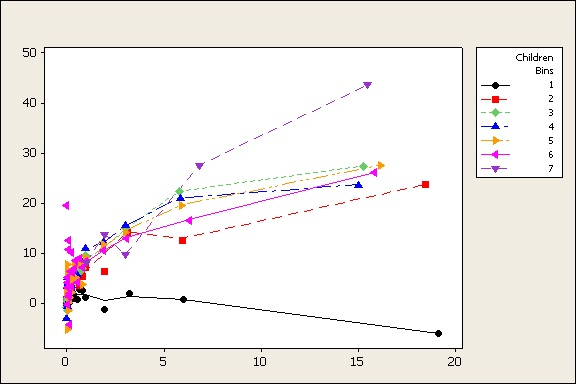
\includegraphics[width=\textwidth]{chapters/chapter_exec_models/figures/fig7.jpg}
        \end{minipage}
    \caption{MI vs RS with other factors. \label{fig:mivsrs}}
    \end{figure}


Table~\ref{fig:mivsrs} shows the results of power-law models ; the standard errors are shown in parentheses below the estimated regression coefficients. All coefficients in the models presented in Table~\ref{fig:mivsrs} are statistically significant. This is consistent with Almgren et al. (2005)~\cite{athl}, except that in their model the market-cap-to-volume ratio is not significant. It should be noted that the values of $R$-square are significantly higher than other published studies, mainly due to binning and smoothing. The response variable is not an individual parent trade cost, but rather the average cost for trades in a bin representing a combination of various levels of predictors. Thus, the models developed here are intended to predict the average MI for a combination of predictors.
        \begin{table}[!ht]
        \caption{Response Variable is MI (bps) ($\hat{\sigma}^2=225, n=2,$ 211 bins) \label{tab:responsevarmi}}
        \begin{tabular}{|c|c|c|c|c|c|c|}
        Predictor & Model 1& Model 2 & Model 3 & Model 4 & Model 5 & Model 6* \\ \hline
        Rel. Size & 0.53 & 0.51 & 0.56 & 0.63 & 0.43 & \\
        	& (0.02) & (0.02) & (0.02) & (0.02) & (0.02) & \\
        Volatility & & 1.12 & 0.92 & 1.17 & 0.53 & \\
        	& & (0.09) & (0.09) & (0.11) & (0.1) & \\
        Duration	& & & $-0.24$ & $-0.25$ & $-0.47$ & $-0.27$ \\
        	& & & (0.02) & (0.02) & (0.3) & (0.1) \\
        Market Cap & & & & $-0.09$ & $-0.12$ & $-0.04$ \\
        	& & & & (0.02) & (0.02) & (0.07) \\
        No. of Children & & & & & 0.53 & 0.55 \\
        	& & & & & (0.04) & (0.16) \\
        Constant & 9.6 & 19.6 & 15.9 & 9.4 & 2.7 & 1.3 \\
        	& (0.34) & (1.07) & (0.9) & (1.3) & (0.46) & (1.3) \\ \hline
        $\hat{\sigma}_{\text{error}}^2$ & 143 & 136 & 125 & 124 & 114 & N/A \\
        $R^2$ & 0.37 & 0.40 & 0.45 & 0.45 & 0.50 & 0.03 \\
        \end{tabular}
        {\small*Response Variable $= \frac{\text{MI}(\text{bps})}{(\text{Vol})(\text{RS})^{0.6}}$}
        \end{table}
Building empirical models for noisy data almost always requires some smoothing of raw data. While there are excellent methods such as kernel smoothing, smoothing in a higher dimension is not easy due to `curse of dimensionality' problem. Thus, we chose this simple approach of binning. 


Several relevant observations can be made about the coefficients in the estimated models. For example, Model~3, which is traditionally well cited in the literature, can be written as:
	\[
	\text{MI(\text{bps})}= 15.9 \cdot \sigma^{0.92} \cdot(RS)^{0.56} \cdot T^{-0.24}.
	\]
Note that the volatility coefficient is approximately `one' and the coefficient of RS is about 0.5 has indeed been observed in the literature. It is consistent with the folklore that it takes one day's volatility to trade one day's volume. The duration effect is also consistent as most of the parent trading occurs in less than two hours in the data set, not always in real life. This has led us to consider an additional model where $\frac{\text{MI(bps)}}{(\text{Vol})(\text{RS})^{0.6}}$ is used as a normalized response variable. This variable can be taken as the multiplicative residual term of  Model (2) in Table~\ref{fig:marketimpt}.The regression results of this variable on other variables are given under Model (6$^*$). Two observations can be made: the duration and the number of child trades are still significant factors. However, the increase in $R$-square is somewhat smaller than the unrestricted versions of the same model, labeled as Model (5) in Table~\ref{fig:marketimpt}.


Other key findings can be summarized as follows:
        \begin{itemize}
        \item Relative size (RS) and volatility ($\sigma$) consistently exhibit positive influences on MI; their impact varies depending on other factors in the model.
        \item Duration ($T$) has an inverse effect. Its use in the model must be carefully calibrated as the execution of parent trades using child trades can be highly concentrated.
        \item Stocks with higher market capitalizations tend to have smaller price impact for the same relative size.
        \item The number of child trades, which is usually determined by the trading algorithm, does reveal a positive effect on MI.
        \end{itemize}
There are several practical considerations that may limit the use of these model for pre-trade cost estimation. These challenges in MI calibration is due to the following facts:
	\begin{enumerate}[--]
	\item Not enough data for certain combinations of the factors involved.
	\item MI is a noisy measure which is hard to calibrate ex-post.
	\item Sometimes, market moves at a much larger magnitude than MI.
	\item Use of raw data results in a poor predictive models; thus a need for aggregation. But aggregation obviously ignores the wide variation within the aggregated unit. 
	\end{enumerate}